\begin{XeClass}{FsServerDefaults}
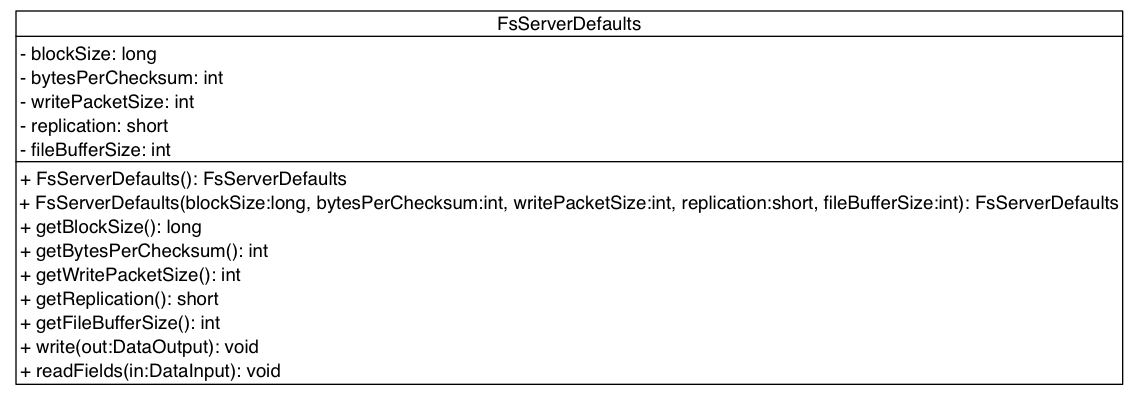
\includegraphics[width=\textwidth]{cdig/FsServerDefaults.png}
     
 文件系统默认服务器类,
 向客户端提供服务器的默认相关设置参数,包括数据块的大小,
 校验和的位数,Packet的大小,文件的副本的数量,
 文件缓冲区的大小

    \begin{XeMethod}{\XePublic}{void}{write}
         
 将服务器的参数值写到输出缓存中

    \end{XeMethod}

    \begin{XeMethod}{\XePublic}{void}{readFields}
         
 读入服务器的各参数值

    \end{XeMethod}

\end{XeClass}
